% Ecosystem and Distribution
% Focus: Marketplace and community approach

\lettrine{T}{he} Symphony extension ecosystem represents more than a traditional software marketplace - it embodies a \textcolor{brandPrimary}{community-driven innovation platform} that balances creator freedom with user safety and system quality.

\subsection*{The Grand Stage Marketplace}

Symphony's marketplace, known as The Grand Stage, serves as the primary distribution channel for community and commercial extensions. The marketplace design prioritizes several key principles:

\begin{description}[leftmargin=3cm,labelwidth=2.5cm]
    \item[\textbf{Discovery}] Intelligent categorization and search capabilities help users find relevant extensions
    \item[\textbf{Trust}] Complete review processes and security scanning build user confidence
    \item[\textbf{Quality}] Performance monitoring and user feedback drive continuous improvement
    \item[\textbf{Sustainability}] Multiple monetization models support extension creator businesses
\end{description}

\subsection*{Security and Trust Framework}

Symphony implements a \textcolor{brandSecondary}{multi-layered security approach} that protects users while enabling innovation:

\begin{table}[ht]
\centering
\begin{tabular}{@{}lll@{}}
\toprule
\textbf{Security Layer} & \textbf{Mechanism} & \textbf{Protection} \\
\midrule
Sandboxed Execution & Process isolation & Fault containment \\
Permission System & Capability-based access & Resource protection \\
Code Review & Automated and manual scanning & Vulnerability prevention \\
Runtime Monitoring & Behavioral analysis & Anomaly detection \\
\bottomrule
\end{tabular}
\caption{Multi-Layer Security Framework}
\end{table}

This approach enables users to confidently install and use community extensions without compromising system security or stability.

\subsection*{Community Governance}

The extension ecosystem operates under a \textcolor{brandAccent}{balanced governance model} that encourages innovation while maintaining quality standards:

\begin{infobox}[title=Governance Principles]
\begin{compactlist}
    \item \textbf{Open Development}: Complete SDKs and documentation enable broad participation
    \item \textbf{Quality Standards}: Automated testing and review processes ensure reliability
    \item \textbf{Community Feedback}: User ratings and reviews guide extension improvement
    \item \textbf{Creator Support}: Technical assistance and business guidance for extension developers
\end{compactlist}
\end{infobox}

\subsection*{Economic Model}

Symphony supports multiple monetization strategies to create a sustainable ecosystem for extension creators:

\begin{compactlist}
    \item \textbf{Free and Open Source}: Community-driven development and reputation building
    \item \textbf{Freemium}: Basic functionality free with premium features available
    \item \textbf{Usage-Based}: Pricing tied to actual consumption of resources or API calls
    \item \textbf{Subscription}: Regular access fees for ongoing value delivery
    \item \textbf{Enterprise Licensing}: Custom arrangements for organizational deployments
\end{compactlist}

This diversity of models accommodates different types of extensions and creator business strategies while providing users with appropriate pricing options.

\subsection*{Enterprise Integration}

Organizations can extend the public marketplace with private extension capabilities:

\begin{description}[leftmargin=4cm,labelwidth=3.5cm]
    \item[\textbf{Private Registries}] Internal-only extensions for proprietary workflows
    \item[\textbf{Access Control}] Role-based permissions for extension installation and usage
    \item[\textbf{Compliance}] Audit trails and governance controls for regulated environments
    \item[\textbf{Custom Development}] Professional services for specialized extension creation
\end{description}

\subsection*{Extension Installation State Management}
\addcontentsline{toc}{subsection}{Extension Installation State Management}

Our research contributes a comprehensive installation state machine that manages the complete extension installation process from marketplace browsing through successful deployment. This state machine provides systematic dependency resolution, security validation, and rollback capabilities for reliable extension management.

\begin{figure}[h]
\centering
% Extension Installation State Management would go here when diagram becomes available
\caption{Extension Installation State Machine showing the complete installation lifecycle management. The system manages eight distinct states: Browsing, Downloading, Verifying, ResolvingDeps, Installing, Installed, RollingBack, and Failed, with comprehensive security validation, dependency resolution, and automatic rollback capabilities for reliable extension deployment.}
\label{fig:extension-installation-states}
\end{figure}

The extension installation state machine addresses critical deployment challenges:

\begin{expandedlist}
    \item \textbf{Security Validation}: Comprehensive signature verification, integrity checks, and malware scanning
    \item \textbf{Dependency Resolution}: Automatic dependency detection with semantic versioning and conflict resolution
    \item \textbf{Rollback Capability}: Complete rollback mechanism for failed installations with state restoration
    \item \textbf{User Experience}: Seamless installation process with detailed progress feedback and error reporting
\end{expandedlist}

\begin{center}
\begin{tabular}{@{}lll@{}}
\toprule
\textbf{Installation State} & \textbf{Validation Requirements} & \textbf{Recovery Strategy} \\
\midrule
Browsing & User selection validation & Return to marketplace \\
Downloading & Network connectivity, package integrity & Retry with exponential backoff \\
Verifying & Signature validation, malware scan & Reject and report security issues \\
ResolvingDeps & Semantic versioning, conflict detection & Auto-download or report conflicts \\
Installing & File system operations, registration & Rollback partial installation \\
RollingBack & State restoration, cleanup & Detailed error logging \\
\bottomrule
\end{tabular}
\captionof{table}{Extension Installation State Management}
\end{center}

\subsection*{Developer Experience}

Symphony prioritizes developer experience to encourage high-quality extension creation. The complete extension ecosystem management infrastructure is illustrated in Figure~\ref{fig:orchestra-kit-ecosystem}, which shows how the Orchestra Kit manages the entire extension lifecycle from development through distribution.

\begin{figure}[h]
\centering
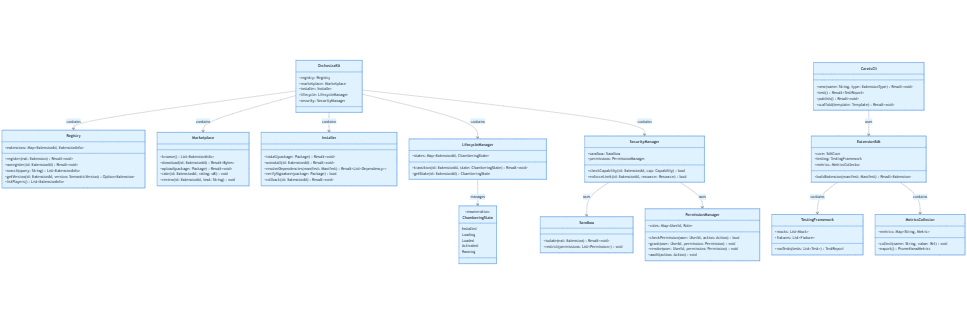
\includegraphics[width=0.9\textwidth]{images/diagrams/class_diagram/4_orchestra_kit_extension_ecosystem.png}
\caption{Orchestra Kit Extension Ecosystem Class Diagram showing the complete extension lifecycle management system including Registry, Marketplace, Installer, Lifecycle Manager, Security Manager, and the Carets CLI/SDK toolchain. This diagram illustrates how all components work together to provide a comprehensive extension development and distribution platform.}
\label{fig:orchestra-kit-ecosystem}
\end{figure}

As shown in the Orchestra Kit architecture, the developer experience encompasses:

\begin{alertbox}
The extension development process is designed to be accessible to developers with varying levels of experience, from individual contributors to large development teams.
\end{alertbox}

Key developer experience features include:

\begin{compactlist}
    \item Complete SDKs for Python, JavaScript/TypeScript, and Rust
    \item Local development and testing environments that mirror production
    \item Automated publishing and distribution workflows
    \item Analytics and feedback systems for understanding extension usage
    \item Community forums and support channels for collaboration and assistance
\end{compactlist}

\subsection*{Ecosystem Growth Strategy}

Symphony's approach to ecosystem growth emphasizes organic community development supported by platform capabilities:

\begin{successbox}
The extension ecosystem is designed to grow through community innovation rather than top-down feature development, enabling Symphony to evolve rapidly in response to user needs and technological advances.
\end{successbox}

This strategy positions Symphony as a platform that becomes more valuable as the community grows, creating positive feedback loops that benefit all participants in the ecosystem.
